\section{Introducción}



\subsection{Motivación de la investigación}

\begin{frame}
    \frametitle{Aplicaciones web}

    \begin{flushleft}
        \begin{tabular}{cccc}
            
\includegraphics[height=1.25cm]{images/itau-logo.png}
            & 
\includegraphics[height=1.25cm]{images/marangatu-logo.jpg}
            & 
\includegraphics[height=1.25cm]{images/facebook-logo.png}
            & 
\includegraphics[height=1.25cm]{images/gmail-logo.jpg}
        \end{tabular}
    \end{flushleft}

    \begin{itemize}
        \item
        Propiedades:

        \begin{itemize}
            % https://blog.sitelock.com/2016/05/web-application-security/

            \item
            Ubicuidad % y accesibilidad
            % Web applications are everywhere and are accessible to cybercriminals
            % 24 hours a day, 7 days a week.

            \item
            Acceso anónimo
            % Since everything is digital, stealthy cybercriminals can anonymously
            % perform attacks without being traced.

            \item
            Código escrito por no expertos
            % Web developers often create custom code for web applications.
            % These custom applications may not be adequately secured, making
            % matters easier for the attacker.

            \item
            Vulnerabilidades presentes
            % Acunetix report 2016

        \end{itemize}
    \end{itemize}
\end{frame}

\begin{frame}[t]
    \frametitle{Vulnerabilidades en aplicaciones web\footnote{
        Acunetix Web Application Vulnerability Report 2016
        \textit{(Datos entre abril 2015 y marzo 2016)}}}

    \begin{columns}
        \column{0.5\textwidth}
        \vspace{-0.4cm}
        \begin{center}
            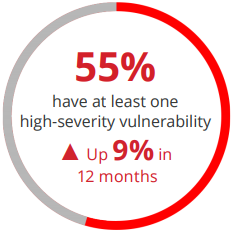
\includegraphics[width=0.8\textwidth]{images/acunetix_vuln_report-1.png}
        \end{center}

        \vspace{-0.5cm}
        \begin{itemize}
            \item
            Severidad alta:
            \textit{Cross-Site Scripting} (XSS), Inyección SQL, entre otros
        \end{itemize}

        \column{0.5\textwidth}
        \vspace{-0.4cm}
        \begin{center}
            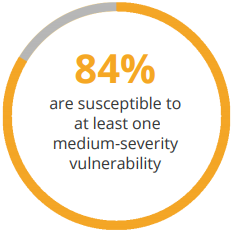
\includegraphics[width=0.8\textwidth]{images/acunetix_vuln_report-2.png}
        \end{center}

        \vspace{-0.5cm}
        \begin{itemize}
            \item
            Severidad media:
            CSRF, Denegación de servicio (DoS), entre otros
        \end{itemize}
    \end{columns}
\end{frame}

\begin{frame}
    \begin{block}{Problema:}
        \begin{itemize}
            \item
            Las aplicaciones web contienen vulnerabilidades y están
            expuestas a un elevado riesgo de ataques.
        \end{itemize}
    \end{block}

    \uncover<2->{
        \begin{block}{Nuestra investigación:}
            \begin{itemize}
                \item
                Mitigación del riesgo de ataques
            \end{itemize}
        \end{block}
    }
\end{frame}

\begin{frame}
    \frametitle{Nuestra investigación}

    \begin{itemize}
        \item
        Web Application Firewall (WAF)

        \begin{itemize}[<.->]
            \item
            Finalidad: mitigar riesgo de ataques
        \end{itemize}
    \end{itemize}

    \begin{center}
        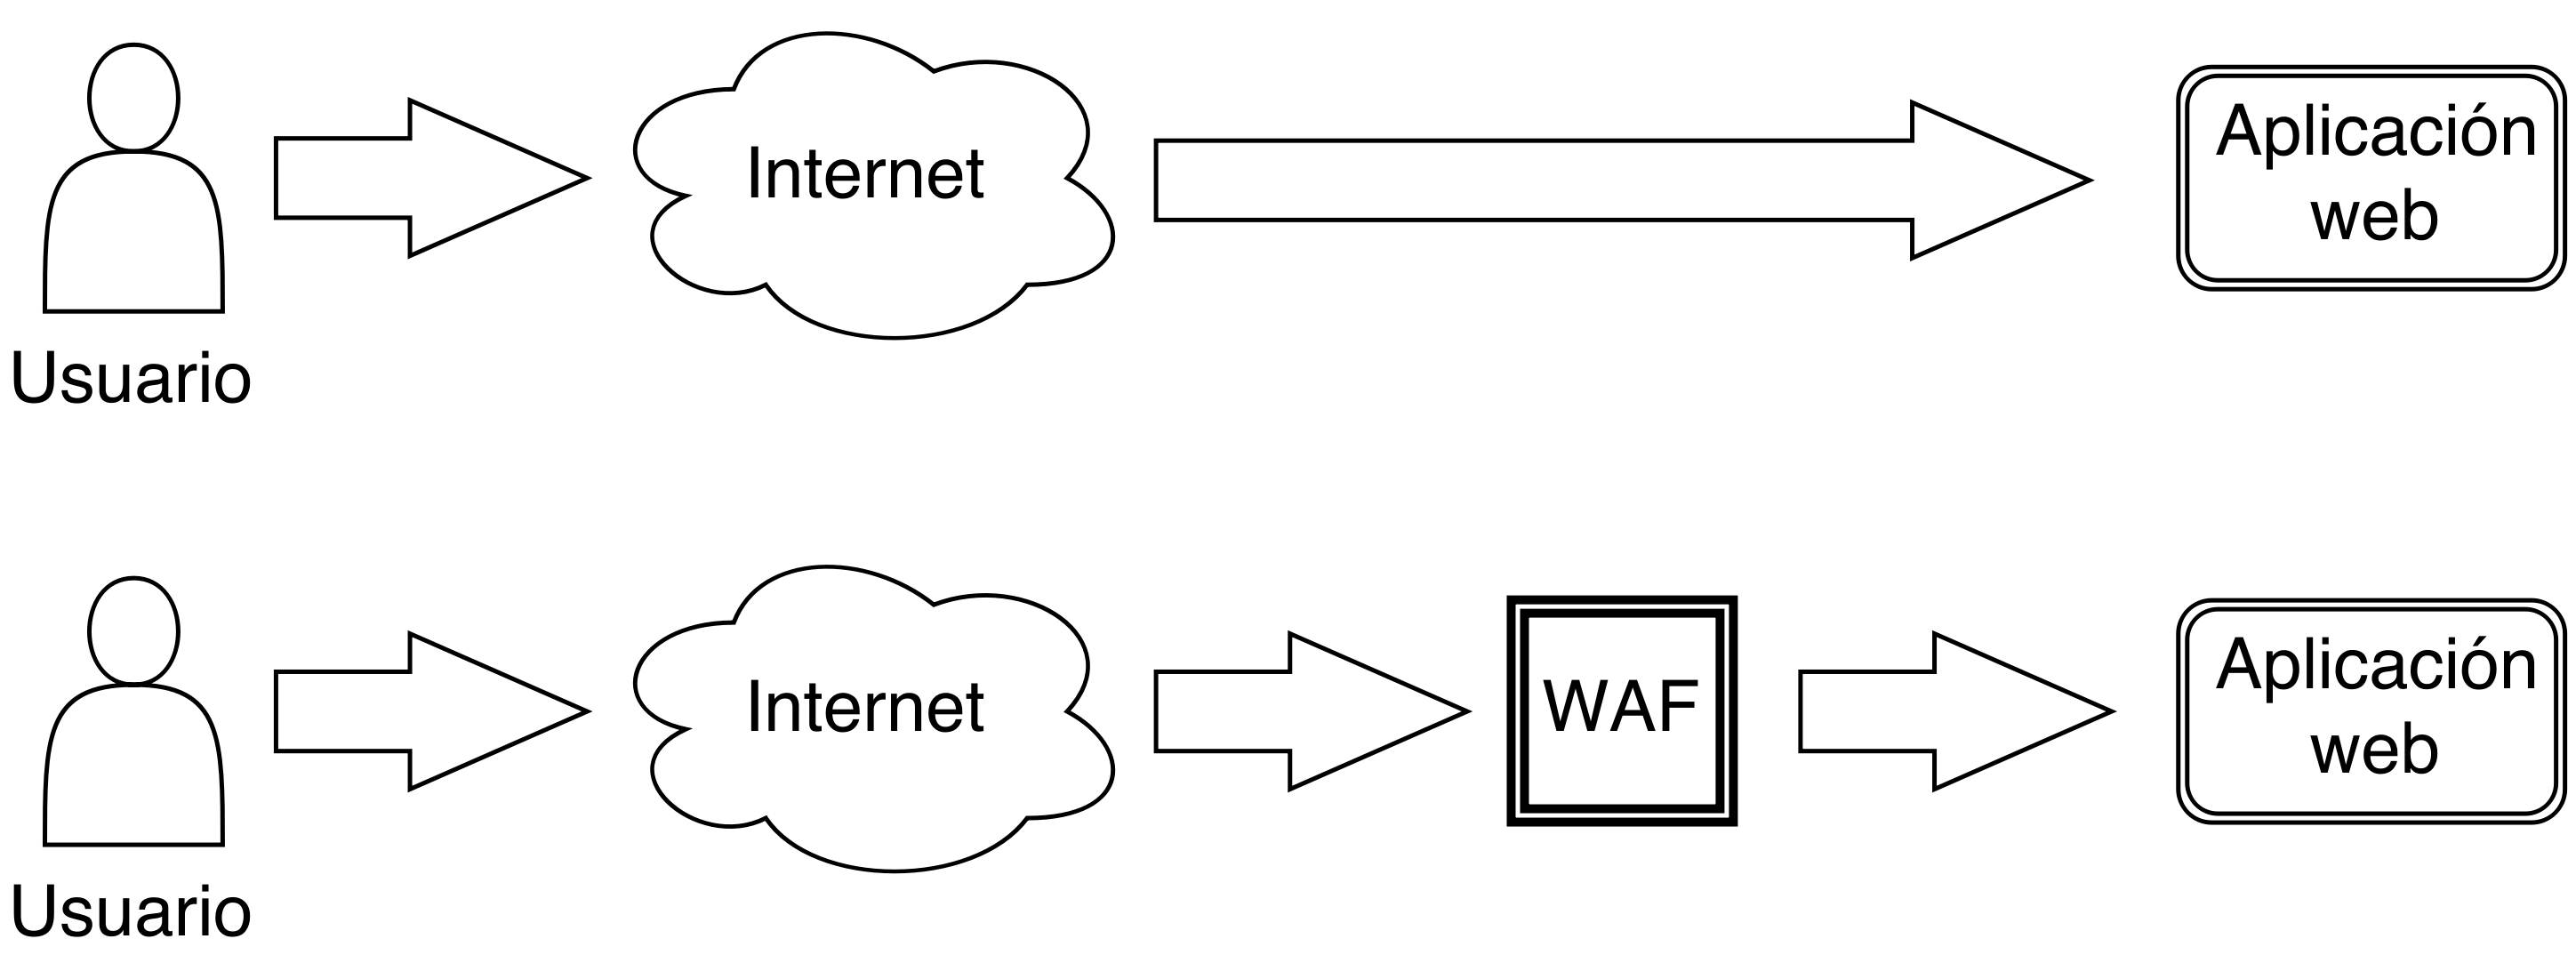
\includegraphics[width=\textwidth]{images/web-app.png}
    \end{center}
\end{frame}

\begin{frame}
    \begin{exampleblock}{Sistemas de Deteción de Intrusiones (IDS)}
        \begin{itemize}
            \item<2->
            Modo de respuesta:

            \begin{itemize}[<.->]
                \item
                Pasivo - detección (IDS)

                \item
                \alert{Activo - prevención (IPS)}
            \end{itemize}

            \item<3->
            Fuente de datos:

            \begin{itemize}[<.->]
                \item
                \textit{Host-based systems} (HIDS)

                \item
                \alert{\textit{Network-based systems} (NIDS)}

                \begin{itemize}
                    \item
                    \alert{Mensajes HTTP $\quad \rightarrow \quad$ WAF}
                \end{itemize}
            \end{itemize}

            \item<4->
            Método de detección:

            \begin{itemize}[<.->]
                \item
                Por firmas de ataques

                \item
                \alert{Por anomalías}
            \end{itemize}
        \end{itemize}
    \end{exampleblock}
\end{frame}

\begin{frame}
    \begin{exampleblock}{WAF con deteción de anomalías}
        \begin{itemize}
            \item<1->
            Dos fases:

            \begin{itemize}[<.->]
                \item
                Fase de entrenamiento: construcción de modelos que describen
                mensajes HTTP normales

                \item
                Fase de detección: comparación de nuevos mensajes con
                modelos construidos
            \end{itemize}

            \item<2->
            Ventaja: detección de ataques nuevos sin re-entrenar

            \item<2->
            Desventaja: dificultad de construir modelos útiles para la detección

            \item<3->
            Estrategías de abordaje:

            \begin{itemize}[<.->]
                \item
                Métodos estadísticos (definición de \textit{threshold})

                \item
                \alert{Problema de clasificación utilizando herramientas de
                \textit{Machine Learning}}
            \end{itemize}
        \end{itemize}
    \end{exampleblock}
\end{frame}

\begin{frame}
    \begin{exampleblock}{Problemas de clasificación y \textit{Machine Learning}}
        \begin{columns}
            \column{0.4\textwidth}
            \begin{center}
                \only<2>{
                    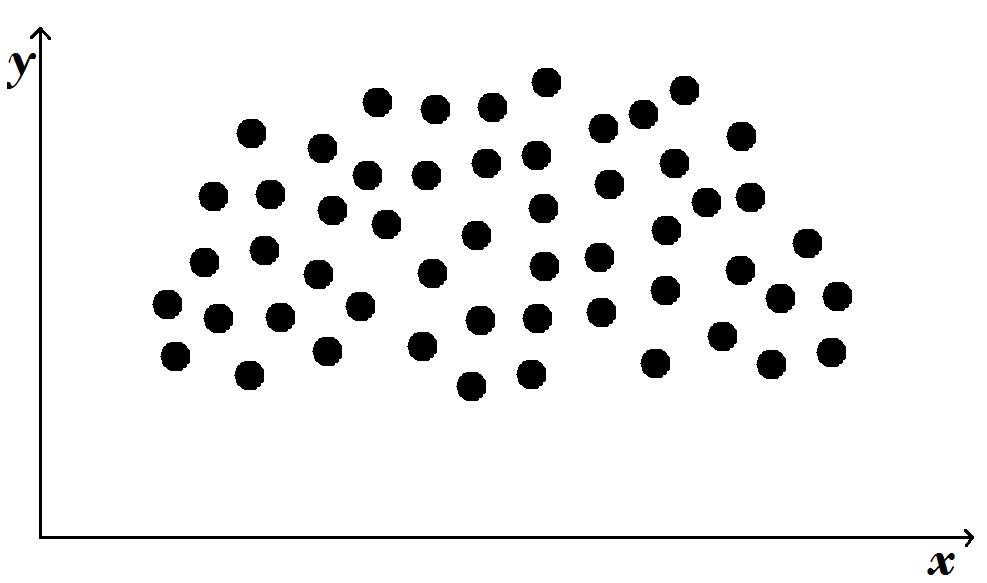
\includegraphics[width=\textwidth]{images/clasif-unsupervised.png}
                }
                \only<3>{
                    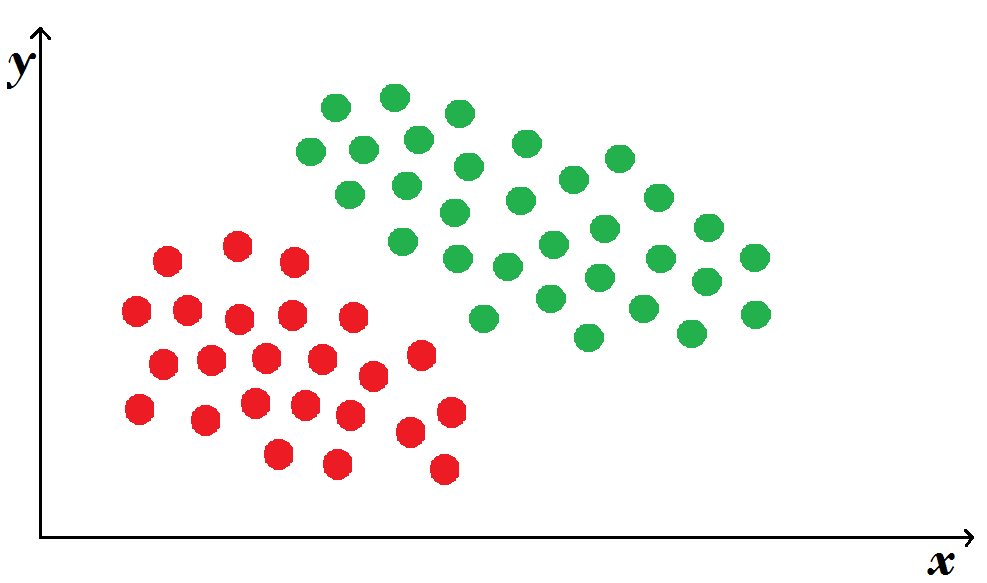
\includegraphics[width=\textwidth]{images/clasif-supervised.png}
                }
                \only<4>{
                    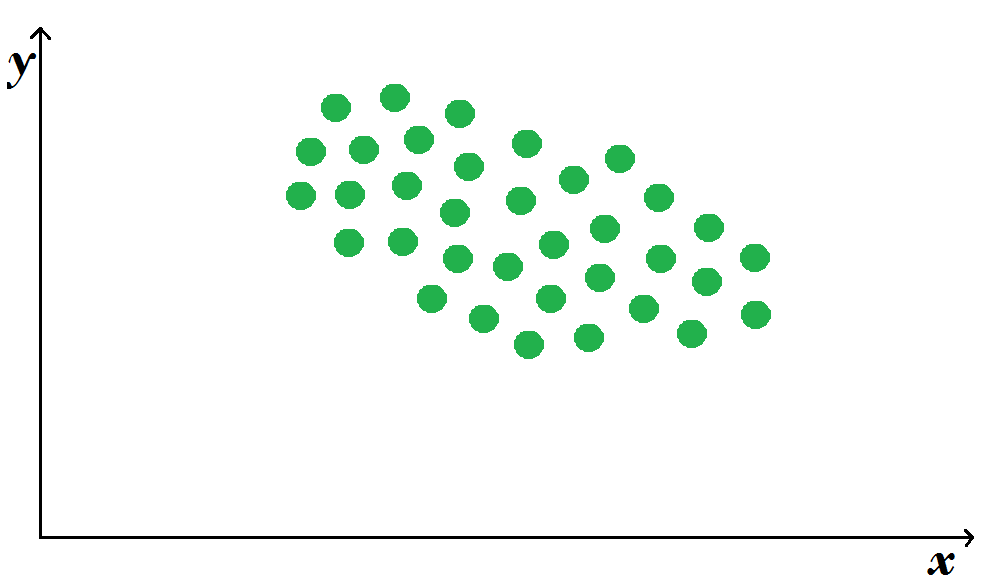
\includegraphics[width=\textwidth]{images/clasif-semi-supervised.png}
                }
            \end{center}

            \column{0.6\textwidth}
            \begin{itemize}[<+(1)->]
                \item
                Clasificación no supervisada

                \item
                Clasificación supervisada

                \item
                Clasificación semi-supervisada

                \begin{itemize}[<.->]
                    \item
                    Caso especial: entrenamiento con muestras de una sola clase
                    OCC: \textit{One-Class Classification}

                    \item
                    Una herramienta posible: One-Class SVM
                \end{itemize}
            \end{itemize}
        \end{columns}
    \end{exampleblock}
\end{frame}



\subsection{Objetivos para la investigación}

\begin{frame}
    \frametitle{Objetivo general}

    \begin{itemize}[<+(1)->]
        \item
        Detectar mensajes HTTP anómalos entre las aplicaciones web y
        sus usuarios con el fin de mitigar los riesgos de ataques contra
        dichas aplicaciones, utilizando un WAF basado en clasificadores
        One-Class SVM.
    \end{itemize}
\end{frame}

\begin{frame}
    \frametitle{Objetivos específicos}

    \begin{enumerate}[<+(1)->]
        \item
        Diseñar procesos de extracción de características (\textit{features})
        específicamente para mensajes HTTP, basado en aportes de otros
        investigadores de la literatura.

        \item
        Implementar un WAF basado en anomalías, utilizando los procesos de
        extracción de \textit{features} diseñados junto con clasificadores
        One-Class SVM.

        \item
        Evaluar la eficacia del WAF implementado en cuanto a la detección
        de mensajes HTTP anómalos.

        \item
        Analizar la viabilidad de utilizar el WAF implementado para
        detección de ataques en tiempo real.
    \end{enumerate}
\end{frame}
